% Options for packages loaded elsewhere
\PassOptionsToPackage{unicode}{hyperref}
\PassOptionsToPackage{hyphens}{url}
%
\documentclass[
  english,
  man,floatsintext]{apa6}
\usepackage{amsmath,amssymb}
\usepackage{lmodern}
\usepackage{ifxetex,ifluatex}
\ifnum 0\ifxetex 1\fi\ifluatex 1\fi=0 % if pdftex
  \usepackage[T1]{fontenc}
  \usepackage[utf8]{inputenc}
  \usepackage{textcomp} % provide euro and other symbols
\else % if luatex or xetex
  \usepackage{unicode-math}
  \defaultfontfeatures{Scale=MatchLowercase}
  \defaultfontfeatures[\rmfamily]{Ligatures=TeX,Scale=1}
\fi
% Use upquote if available, for straight quotes in verbatim environments
\IfFileExists{upquote.sty}{\usepackage{upquote}}{}
\IfFileExists{microtype.sty}{% use microtype if available
  \usepackage[]{microtype}
  \UseMicrotypeSet[protrusion]{basicmath} % disable protrusion for tt fonts
}{}
\makeatletter
\@ifundefined{KOMAClassName}{% if non-KOMA class
  \IfFileExists{parskip.sty}{%
    \usepackage{parskip}
  }{% else
    \setlength{\parindent}{0pt}
    \setlength{\parskip}{6pt plus 2pt minus 1pt}}
}{% if KOMA class
  \KOMAoptions{parskip=half}}
\makeatother
\usepackage{xcolor}
\IfFileExists{xurl.sty}{\usepackage{xurl}}{} % add URL line breaks if available
\IfFileExists{bookmark.sty}{\usepackage{bookmark}}{\usepackage{hyperref}}
\hypersetup{
  pdftitle={Peekbank: Exploring children's word recognition through an open, large-scale repository for developmental eye-tracking data},
  pdfauthor={Peekbank team2, Martin Zettersten1, Claire Bergey2, Naiti S. Bhatt3, Veronica Boyce4, Mika Braginsky5, Alexandra Carstensen4, Benny deMayo1, George Kachergis4, Molly Lewis6, Bria Long4, Kyle MacDonald7, Jessica Mankewitz4, Stephan Meylan5,8, Annissa N. Saleh9, Rose M. Schneider10, Angeline Sin Mei Tsui4, Sarp Uner8, Tian Linger Xu11, Daniel Yurovsky6, \& Michael C. Frank1},
  pdflang={en-EN},
  pdfkeywords={tools; processing; analysis / usage examples},
  hidelinks,
  pdfcreator={LaTeX via pandoc}}
\urlstyle{same} % disable monospaced font for URLs
\usepackage{color}
\usepackage{fancyvrb}
\newcommand{\VerbBar}{|}
\newcommand{\VERB}{\Verb[commandchars=\\\{\}]}
\DefineVerbatimEnvironment{Highlighting}{Verbatim}{commandchars=\\\{\}}
% Add ',fontsize=\small' for more characters per line
\usepackage{framed}
\definecolor{shadecolor}{RGB}{248,248,248}
\newenvironment{Shaded}{\begin{snugshade}}{\end{snugshade}}
\newcommand{\AlertTok}[1]{\textcolor[rgb]{0.94,0.16,0.16}{#1}}
\newcommand{\AnnotationTok}[1]{\textcolor[rgb]{0.56,0.35,0.01}{\textbf{\textit{#1}}}}
\newcommand{\AttributeTok}[1]{\textcolor[rgb]{0.77,0.63,0.00}{#1}}
\newcommand{\BaseNTok}[1]{\textcolor[rgb]{0.00,0.00,0.81}{#1}}
\newcommand{\BuiltInTok}[1]{#1}
\newcommand{\CharTok}[1]{\textcolor[rgb]{0.31,0.60,0.02}{#1}}
\newcommand{\CommentTok}[1]{\textcolor[rgb]{0.56,0.35,0.01}{\textit{#1}}}
\newcommand{\CommentVarTok}[1]{\textcolor[rgb]{0.56,0.35,0.01}{\textbf{\textit{#1}}}}
\newcommand{\ConstantTok}[1]{\textcolor[rgb]{0.00,0.00,0.00}{#1}}
\newcommand{\ControlFlowTok}[1]{\textcolor[rgb]{0.13,0.29,0.53}{\textbf{#1}}}
\newcommand{\DataTypeTok}[1]{\textcolor[rgb]{0.13,0.29,0.53}{#1}}
\newcommand{\DecValTok}[1]{\textcolor[rgb]{0.00,0.00,0.81}{#1}}
\newcommand{\DocumentationTok}[1]{\textcolor[rgb]{0.56,0.35,0.01}{\textbf{\textit{#1}}}}
\newcommand{\ErrorTok}[1]{\textcolor[rgb]{0.64,0.00,0.00}{\textbf{#1}}}
\newcommand{\ExtensionTok}[1]{#1}
\newcommand{\FloatTok}[1]{\textcolor[rgb]{0.00,0.00,0.81}{#1}}
\newcommand{\FunctionTok}[1]{\textcolor[rgb]{0.00,0.00,0.00}{#1}}
\newcommand{\ImportTok}[1]{#1}
\newcommand{\InformationTok}[1]{\textcolor[rgb]{0.56,0.35,0.01}{\textbf{\textit{#1}}}}
\newcommand{\KeywordTok}[1]{\textcolor[rgb]{0.13,0.29,0.53}{\textbf{#1}}}
\newcommand{\NormalTok}[1]{#1}
\newcommand{\OperatorTok}[1]{\textcolor[rgb]{0.81,0.36,0.00}{\textbf{#1}}}
\newcommand{\OtherTok}[1]{\textcolor[rgb]{0.56,0.35,0.01}{#1}}
\newcommand{\PreprocessorTok}[1]{\textcolor[rgb]{0.56,0.35,0.01}{\textit{#1}}}
\newcommand{\RegionMarkerTok}[1]{#1}
\newcommand{\SpecialCharTok}[1]{\textcolor[rgb]{0.00,0.00,0.00}{#1}}
\newcommand{\SpecialStringTok}[1]{\textcolor[rgb]{0.31,0.60,0.02}{#1}}
\newcommand{\StringTok}[1]{\textcolor[rgb]{0.31,0.60,0.02}{#1}}
\newcommand{\VariableTok}[1]{\textcolor[rgb]{0.00,0.00,0.00}{#1}}
\newcommand{\VerbatimStringTok}[1]{\textcolor[rgb]{0.31,0.60,0.02}{#1}}
\newcommand{\WarningTok}[1]{\textcolor[rgb]{0.56,0.35,0.01}{\textbf{\textit{#1}}}}
\usepackage{graphicx}
\makeatletter
\def\maxwidth{\ifdim\Gin@nat@width>\linewidth\linewidth\else\Gin@nat@width\fi}
\def\maxheight{\ifdim\Gin@nat@height>\textheight\textheight\else\Gin@nat@height\fi}
\makeatother
% Scale images if necessary, so that they will not overflow the page
% margins by default, and it is still possible to overwrite the defaults
% using explicit options in \includegraphics[width, height, ...]{}
\setkeys{Gin}{width=\maxwidth,height=\maxheight,keepaspectratio}
% Set default figure placement to htbp
\makeatletter
\def\fps@figure{htbp}
\makeatother
\setlength{\emergencystretch}{3em} % prevent overfull lines
\providecommand{\tightlist}{%
  \setlength{\itemsep}{0pt}\setlength{\parskip}{0pt}}
\setcounter{secnumdepth}{-\maxdimen} % remove section numbering
% Make \paragraph and \subparagraph free-standing
\ifx\paragraph\undefined\else
  \let\oldparagraph\paragraph
  \renewcommand{\paragraph}[1]{\oldparagraph{#1}\mbox{}}
\fi
\ifx\subparagraph\undefined\else
  \let\oldsubparagraph\subparagraph
  \renewcommand{\subparagraph}[1]{\oldsubparagraph{#1}\mbox{}}
\fi
% Manuscript styling
\usepackage{upgreek}
\captionsetup{font=singlespacing,justification=justified}

% Table formatting
\usepackage{longtable}
\usepackage{lscape}
% \usepackage[counterclockwise]{rotating}   % Landscape page setup for large tables
\usepackage{multirow}		% Table styling
\usepackage{tabularx}		% Control Column width
\usepackage[flushleft]{threeparttable}	% Allows for three part tables with a specified notes section
\usepackage{threeparttablex}            % Lets threeparttable work with longtable

% Create new environments so endfloat can handle them
% \newenvironment{ltable}
%   {\begin{landscape}\centering\begin{threeparttable}}
%   {\end{threeparttable}\end{landscape}}
\newenvironment{lltable}{\begin{landscape}\centering\begin{ThreePartTable}}{\end{ThreePartTable}\end{landscape}}

% Enables adjusting longtable caption width to table width
% Solution found at http://golatex.de/longtable-mit-caption-so-breit-wie-die-tabelle-t15767.html
\makeatletter
\newcommand\LastLTentrywidth{1em}
\newlength\longtablewidth
\setlength{\longtablewidth}{1in}
\newcommand{\getlongtablewidth}{\begingroup \ifcsname LT@\roman{LT@tables}\endcsname \global\longtablewidth=0pt \renewcommand{\LT@entry}[2]{\global\advance\longtablewidth by ##2\relax\gdef\LastLTentrywidth{##2}}\@nameuse{LT@\roman{LT@tables}} \fi \endgroup}

% \setlength{\parindent}{0.5in}
% \setlength{\parskip}{0pt plus 0pt minus 0pt}

% \usepackage{etoolbox}
\makeatletter
\patchcmd{\HyOrg@maketitle}
  {\section{\normalfont\normalsize\abstractname}}
  {\section*{\normalfont\normalsize\abstractname}}
  {}{\typeout{Failed to patch abstract.}}
\patchcmd{\HyOrg@maketitle}
  {\section{\protect\normalfont{\@title}}}
  {\section*{\protect\normalfont{\@title}}}
  {}{\typeout{Failed to patch title.}}
\makeatother
\shorttitle{Peekbank repository for developmental eye-tracking data}
\keywords{tools; processing; analysis / usage examples\newline\indent Word count: X}
\DeclareDelayedFloatFlavor{ThreePartTable}{table}
\DeclareDelayedFloatFlavor{lltable}{table}
\DeclareDelayedFloatFlavor*{longtable}{table}
\makeatletter
\renewcommand{\efloat@iwrite}[1]{\immediate\expandafter\protected@write\csname efloat@post#1\endcsname{}}
\makeatother
\usepackage{lineno}

\linenumbers
\usepackage{csquotes}
\ifxetex
  % Load polyglossia as late as possible: uses bidi with RTL langages (e.g. Hebrew, Arabic)
  \usepackage{polyglossia}
  \setmainlanguage[]{english}
\else
  \usepackage[main=english]{babel}
% get rid of language-specific shorthands (see #6817):
\let\LanguageShortHands\languageshorthands
\def\languageshorthands#1{}
\fi
\ifluatex
  \usepackage{selnolig}  % disable illegal ligatures
\fi
\newlength{\cslhangindent}
\setlength{\cslhangindent}{1.5em}
\newlength{\csllabelwidth}
\setlength{\csllabelwidth}{3em}
\newenvironment{CSLReferences}[2] % #1 hanging-ident, #2 entry spacing
 {% don't indent paragraphs
  \setlength{\parindent}{0pt}
  % turn on hanging indent if param 1 is 1
  \ifodd #1 \everypar{\setlength{\hangindent}{\cslhangindent}}\ignorespaces\fi
  % set entry spacing
  \ifnum #2 > 0
  \setlength{\parskip}{#2\baselineskip}
  \fi
 }%
 {}
\usepackage{calc}
\newcommand{\CSLBlock}[1]{#1\hfill\break}
\newcommand{\CSLLeftMargin}[1]{\parbox[t]{\csllabelwidth}{#1}}
\newcommand{\CSLRightInline}[1]{\parbox[t]{\linewidth - \csllabelwidth}{#1}\break}
\newcommand{\CSLIndent}[1]{\hspace{\cslhangindent}#1}

\title{Peekbank: Exploring children's word recognition through an open, large-scale repository for developmental eye-tracking data}
\author{Peekbank team\textsuperscript{2}, Martin Zettersten\textsuperscript{1}, Claire Bergey\textsuperscript{2}, Naiti S. Bhatt\textsuperscript{3}, Veronica Boyce\textsuperscript{4}, Mika Braginsky\textsuperscript{5}, Alexandra Carstensen\textsuperscript{4}, Benny deMayo\textsuperscript{1}, George Kachergis\textsuperscript{4}, Molly Lewis\textsuperscript{6}, Bria Long\textsuperscript{4}, Kyle MacDonald\textsuperscript{7}, Jessica Mankewitz\textsuperscript{4}, Stephan Meylan\textsuperscript{5,8}, Annissa N. Saleh\textsuperscript{9}, Rose M. Schneider\textsuperscript{10}, Angeline Sin Mei Tsui\textsuperscript{4}, Sarp Uner\textsuperscript{8}, Tian Linger Xu\textsuperscript{11}, Daniel Yurovsky\textsuperscript{6}, \& Michael C. Frank\textsuperscript{1}}
\date{}


\authornote{

Add complete departmental affiliations for each author here. Each new line herein must be indented, like this line.
Enter author note here.

The authors made the following contributions. Peekbank team: Conceptualization, Writing - Original Draft Preparation, Writing - Review \& Editing.

Correspondence concerning this article should be addressed to Peekbank team, Postal address. E-mail: \href{mailto:my@email.com}{\nolinkurl{my@email.com}}

}

\affiliation{\vspace{0.5cm}\textsuperscript{1} Dept. of Psychology, Princeton University\\\textsuperscript{2} Dept. of Psychology, University of Chicago\\\textsuperscript{3} Scripps College\\\textsuperscript{4} Dept. of Psychology, Stanford University\\\textsuperscript{5} Dept. of Brain and Cognitive Sciences, MIT\\\textsuperscript{6} Dept. of Psychology, Carnegie Mellon University\\\textsuperscript{7} Core Technology, McD Tech Labs\\\textsuperscript{8} Dept. of Psychology and Neuroscience, Duke University\\\textsuperscript{9} Dept. of Psychology, UT Austin\\\textsuperscript{10} Dept. of Psychology, UC San Diego\\\textsuperscript{11} Dept. of Psychological and Brain Sciences, Indiana University}

\abstract{
The ability to rapidly recognize words and link them to referents in context is central to children's early language development.
This ability, often called word recognition in the developmental literature, is typically studied in the looking-while-listening paradigm, which measures infants' fixation on a target object (vs.~a distractor) after hearing a target label.
We present a large-scale, open database of infant and toddler eye-tracking data from looking-while-listening tasks.
The goal of this effort is to address theoretical and methodological challenges in measuring vocabulary development.
}



\begin{document}
\maketitle

\hypertarget{introduction}{%
\section{Introduction}\label{introduction}}

Across their first years of life, children learn words at an accelerating pace (Frank, Braginsky, Yurovsky, \& Marchman, 2021).
Although many children will only produce their first word at around one year of age, they show signs of understanding many common nouns (e.g., ``mommy'') and phrases (e.g., ``Let's go bye-bye!'') much earlier in development (Bergelson \& Swingley, 2012).
However, the processes involved in early word understanding are less directly apparent in children's behaviors and are less accessible to observation than developments in speech production (Fernald, Zangl, Portillo, \& Marchman, 2008).
To understand speech, children must process the incoming auditory signal and link that signal to relevant meanings -- a process often referred to as word recognition.
Measuring early word recognition offers insight into children's early word representations and as well as the speed and efficiency with which children comprehend language in real time, as the speech signal unfolds (Bergelson, 2020; Fernald, Pinto, Swingley, Weinberg, \& McRoberts, 1998).
Word recognition skills are also thought to build a foundation for children's subsequent language development.
Past research has found that early word recognition efficiency is predictive of later linguistic and general cognitive outcomes (Bleses, Makransky, Dale, Højen, \& Ari, 2016; Marchman et al., 2018).
One explanation for this relationship is that efficiency of word recognition facilitates subsequent word learning: the faster children are at processing speech, the more efficiently they can learn from the input in their environment (Fernald \& Marchman, 2012).

While word recognition is a central part of children's language development, mapping the trajectory of word recognition skills has remained elusive. Studies investigating children's word recognition are typically limited in scope to experiments in individual labs involving small samples tested on a limited set of items.
This limitation in scale makes it difficult to understand developmental changes in children's word knowledge at a broad scale.
Peekbank provides an openly accessible database of eye-tracking data of children's word recognition, with the primary goal of facilitating the study of developmental changes in children's word knowledge and recognition speed.

\hypertarget{the-looking-while-listening-paradigm}{%
\subsection{The ``Looking-While-Listening'' Paradigm}\label{the-looking-while-listening-paradigm}}

Word recognition is traditionally studied in the ``looking-while-listening'' paradigm {[}alternatively referred to as the intermodal preferential looking procedure; Fernald, Zangl, Portillo, and Marchman (2008); Hirsh-Pasek, Cauley, Golinkoff, and Gordon (1987){]}.
In such studies, infants listen to a sentence prompting a specific referent (e.g., Look at the dog!) while viewing two images on the screen (e.g., an image of a dog -- the target image -- and an image of a duck -- the distractor image).
Infants' word recognition is measured in terms of how quickly and accurately they fixate on the correct target image after hearing its label.
Past research has used this same basic method to study a wide range of questions in language development.
For example, the looking-while-listening paradigm has been used to uncover early knowledge of nouns in infants' early noun knowledge, phonological representations of words, prediction during language processing, and individual differences in language development (Bergelson \& Swingley, 2012; Golinkoff, Ma, Song, \& Hirsh-Pasek, 2013; Lew-Williams \& Fernald, 2007; Marchman et al., 2018; Swingley \& Aslin, 2000).

\hypertarget{measuring-developmental-change-in-word-recognition}{%
\subsection{Measuring developmental change in word recognition}\label{measuring-developmental-change-in-word-recognition}}

While the looking-while-listening paradigm has been highly fruitful in advancing understanding of early word knowledge, fundamental questions remain both about the trajectory of children's word recognition ability and the nature of the method itself.
One central question is how to measure developmental change in word recognition.
A key idea in the language learning literature is that processing speed - the ability to quickly link a word with its referent - supports language learning.
Age-related changes in speed of processing are thought to accelerate infants' subsequent language learning: the faster infants are able to process incoming speech input, the better able they become to learn from their language environment.

Similarly, longitudinal analyses have found that individual differences in word recognition speed predict linguistic and cognitive outcomes later in childhood (e.g., Marchman \& Fernald, 2008).
However, measuring increases in the speed and accuracy of word recognition faces the challenge of distinguishing developmental changes in word recognition skill from changes in knowledge of specific words.
This problem is particularly thorny in child development, since the number of items that can be tested within a single session is limited and items must be selected in an age-appropriate manner (Peter et al., 2019).
Measuring developmental change therefore requires large-scale datasets with a range of items, in order to generalize age-related changes across words.

\hypertarget{developing-methodological-best-practices}{%
\subsection{Developing methodological best-practices}\label{developing-methodological-best-practices}}

A second question relates to evaluating methodological best practices.
In particular, many fundamental analytic decisions vary substantially across studies, and different decisions may lead to different inferences about children's word recognition.
For example, researchers vary in how they select time windows for analysis, transform the dependent measure of target fixations, and model the time course of word recognition (Csibra, Hernik, Mascaro, Tatone, \& Lengyel, 2016; Fernald, Zangl, Portillo, \& Marchman, 2008; Huang \& Snedeker, 2020).
This problem is made more complex by the fact that many of these decisions depend on a variety of design-related and participant-related factors (e.g., infant age).
Establishing best practices therefore requires a large database of infant word recognition studies varying across such factors, in order to test the potential consequences of methodological decisions on study results.

\hypertarget{peekbank-an-open-database-of-developmental-eye-tracking-studies.}{%
\subsection{Peekbank: An open database of developmental eye-tracking studies.}\label{peekbank-an-open-database-of-developmental-eye-tracking-studies.}}

What these two questions share is that they are difficult to answer at the scale of a single study.
To address this challenge, we introduce Peekbank, a flexible and reproducible interface to an open database of developmental eye-tracking studies.
The Peekbank project (a) collects a large set of eye-tracking datasets on children's word recognition, (b) introduces a data format and processing tools for standardizing eye-tracking data across data sources, and (c) provides an interface for accessing and analyzing the database.
In the current paper, we give an overview of the key components of the project and some initial demonstrations of its utility in advancing theoretical and methodological insights.
We report two analyses using the database and associated tools (N=1,233): (1) a growth curve analysis modeling age-related changes in infants' word recognition while generalizing across item-level variability; and (2) a multiverse-style analysis of how a central methodological decision -- selecting the time window of analysis -- impacts inter-item reliability.

\hypertarget{design-and-technical-approach}{%
\section{Design and Technical Approach}\label{design-and-technical-approach}}

\hypertarget{database-framework}{%
\subsection{Database Framework}\label{database-framework}}

One of the main challenges in compiling a large-scale eye-tracking dataset is the lack of a shared data format across individual experiments.
Researcher conventions for structuring data vary, as do the technical specifications of different devices (e.g., computer displays and eyetracking cameras), rendering the task of integrating datasets from different labs and data sources difficult.
Therefore, our first effort was to develop a common tabular format to support analyses of all studies simultaneously.

As illustrated in Figure \ref{fig:fig-framework-overview}, the Peekbank framework consists of three main components: (1) a set of tools to convert eye-tracking datasets into a unified format; (2) a relational database populated with data in this unified format and (3) a set of tools to retrieve data from this database.
These components are supported by three libraries.
The \texttt{peekds} library (for the R language; (\textbf{rcoreteam2020?}) helps researchers convert existing datasets to use the standardized format of the database.
The \texttt{peekbank} module (Python) creates a database with the relational schema and populates it with the standardized datasets produced by \texttt{peekds}.
The database is implemented in MySQL, an industry standard relational database, which may be accessed by a variety of programming languages, and can be hosted on one machine and accessed by many others over the Internet.
The \texttt{peekbankr} library (R) provides an application programming interface, or API, that offers high-level abstractions for accessing data in Peekbank.
Most users will access data through this final library, in which case the details of data formatting and processing are abstracted away from the user.

In the following sections, we will begin by providing the details on the database's organization (or \textit{schema}) and the technical implementation on \texttt{peekds}.
Users who are primarily interested in accessing the database can skip these details and focus on access through the \texttt{peekbankr} API and the web apps.

\begin{figure}

{\centering 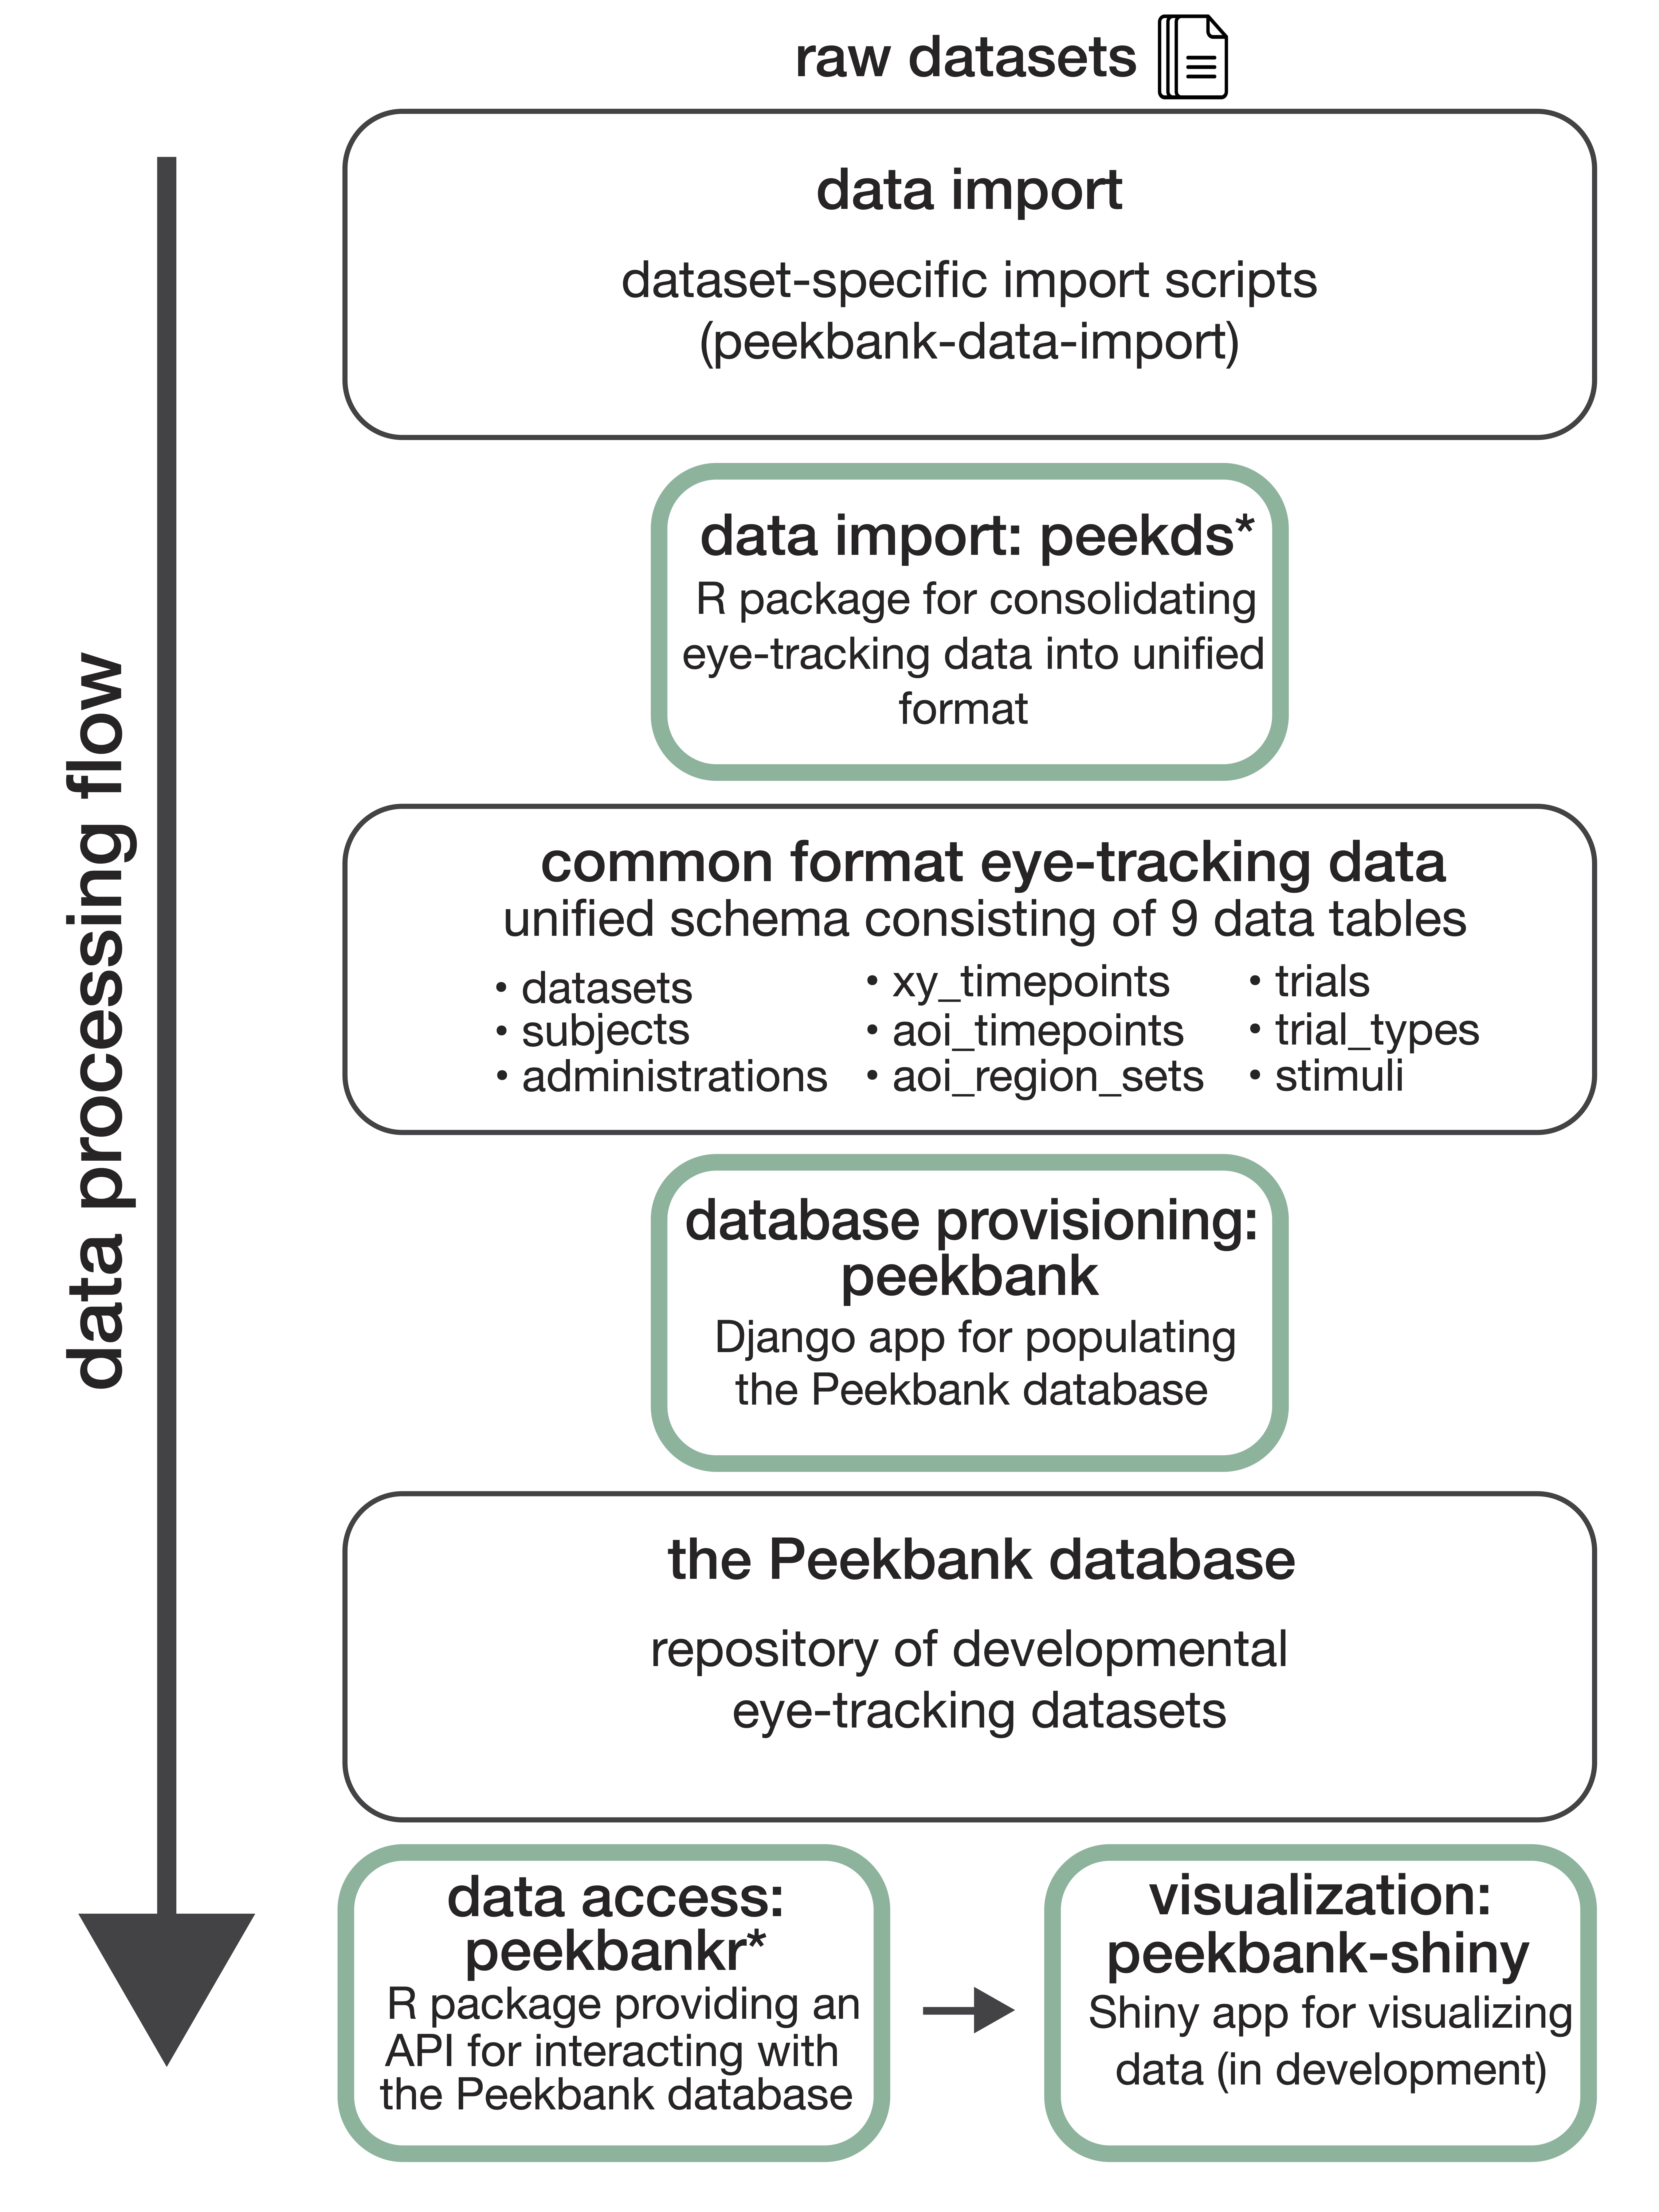
\includegraphics[width=18in,height=4.5in]{/Users/mikabr/Dropbox/projects/peekbank/peekbank-paper/brm/figures/peekbankflowchartv6} 

}

\caption{Overview of the Peekbank data ecosystem. Peekbank tools are highlighted in green. *R packages introduced in this work.}\label{fig:fig-framework-overview}
\end{figure}

\hypertarget{database-schema}{%
\subsection{Database Schema}\label{database-schema}}

The peekbank database contains two major types of data: (1) timecourse looking data, detailing where on the screen a child is looking at a given point in time, or (2) metadata regarding the relevant experiment, participant, and trial (Fig XX).
Here, we will give an outline of the tables encoding this data.
As is common in relational databases, records of similar types (e.g., participants, trials, experiments, coded looks at each timepoint) are grouped into tables, and records of various types are linked through numeric identifiers.

\hypertarget{timecourse-data}{%
\subsubsection{Timecourse data}\label{timecourse-data}}

Timecourse looking data is encoded in two tables: \texttt{aoi\_timepoints} and \texttt{xy\_timepoints}.
The \texttt{aoi\_timepoints} table encodes where a child is looking at each point in time, by specifying the coded area of interest (AOI): looks to the target, looks to the distractor, looks on the screen but away from target and distractor, and missing looks.
All datasets must include this timecourse data, as it represents the main record of children's looking behavior.
For eyetracking experiments that are automatically rather than manually coded, the \texttt{xy\_timepoints} table encodes the inferred (x, y) coordinates of fixations on the screen over the course of each trial.
Both the \texttt{aoi\_timepoints} and \texttt{xy\_timepoints} tables are resampled to a consistent sampling rate, as described in the Import section below.
To normalize across trials and across experiments, all timecourses are computed so that the time of 0 ms represents the onset of disambiguating material (i.e., the beginning of \textit{dog} in ``can you find the \textit{dog}?'').

\hypertarget{metadata}{%
\subsubsection{Metadata}\label{metadata}}

Each record in the timecourse data is linked to several metadata records.
This metadata can be separated into three parts: (1) subject-level information (e.g., demographics) (2) experiment-level information (e.g., a subject's age for a specific experiment, or the particular eyetracker used to collect the data) and (3) trial information and experimental design (what images or videos were presented onscreen, and paired with which audio).
Information about individuals who participate in one more studies, for example a subject's sex and first language, is recorded in the \texttt{subjects} table, while the \texttt{administrations} table contains information about a specific subject participating in a specific experiment.
This division allows Peekbank to gracefully handle longitudinal designs: a single subject can be associated with many administrations.

The \texttt{stimuli} and \texttt{trial\_types} tables store information about trials, which in turn may reflect specifics of the experiment design.
Stimuli are (label, image) mappings that are seen in the experiment.
The \texttt{trial\_types} table encodes information about each trial of the experiment, including the target stimulus and location, the distractor stimulus and location, and the point of disambiguation for that trial.
If this dataset used automatic eyetracking rather than manual coding, each trial type is additionally linked to a set of area of interest (x, y) coordinates, encoded in the \texttt{aoi\_region\_sets} table.

Because individual trial types can be repeated multiple times within an administration, the order of the trials is encoded in the \texttt{trials} table.
Each unique ordering that occurred in the experiment is encoded in this table.
For example, if every participant saw the same ordering, the trials table would only have as many rows as there were trials in the experiment; if there were many different orderings, the trials table would represent each ordering.
The \texttt{trial\_id}, which links a trial type to the order it was presented in an administration, is attached to the time course looking data.

\hypertarget{import}{%
\subsection{Import}\label{import}}

During data import, raw eye-tracking datasets are processed to conform to the Peekbank data schema.
The following section is a description of the import process for peekbank.
It serves as both a description of our method in importing the datasets already in the database, as well as a high-level overview of the import process for researchers looking to import their data in the future.
First, we will describe the import of metadata, and second, we will describe import of the timecourse looking data, including processing functions in \texttt{peekds} for normalizing and resampling looking behavior.

\hypertarget{metadata-1}{%
\subsubsection{Metadata}\label{metadata-1}}

Subject-level data is imported for all participants who have experiment data.
In general, we import data without particular exclusions, including as many participants as possible in the database.
The \texttt{subjects} and \texttt{administrations} tables separate information at the subject level from information about runs of the experiment, such that longitudinal studies have multiple administrations linked to each subject.

The \texttt{stimuli} table has a row for each (word, image) pair, and thus is used slightly differently across different experiment designs.
In most experiments, there is a one-to-one mapping between images and labels (e.g., each time an image of a dog appears it is referred to as ``dog'').
For studies in which there are multiple potential labels per image (e.g., ``dog'' and ``chien'' are both used to refer to an image of a dog), images can have multiple rows in the \texttt{stimuli} table with unique labels as well as a row with no label to be used when the image appears solely as a distractor (and thus its label is ambiguous).
This structure is useful for studies on synonymy or using multiple languages.
For studies in which the same label refers to multiple images (e.g., the word ``dog'' refers to an image of a dalmatian and a poodle), the same label can have multiple rows in the \texttt{stimuli} table with unique images.
The \texttt{trial\_types} table contains each pair of stimuli, a target and distractor, seen in the experiment.
The \texttt{trial\_types} table links trial types to the \texttt{aoi\_region\_sets} table and the \texttt{trials} table.

The \texttt{trials} table encodes each unique ordering of trial types seen in all runs of an experiment.
For example, for experiments with a fixed trial order, the \texttt{trials} table will have as many rows as there are stimuli in the experiment; for experiments with a randomized trial order, there will be many rows linking the trial orderings to the trial types.
The \texttt{trials} table links all experiment design information to the timecourse data.

\hypertarget{timecourse-data-1}{%
\subsubsection{Timecourse data}\label{timecourse-data-1}}

Raw looking data is a series of looks to AOIs or to (x, y) coordinates on the experiment screen, linked to points in time.
For data generated by eyetrackers, we typically have (x, y) coordinates at each time point, which will be encoded in the \texttt{xy\_timepoints} table.
These looks will also be recoded into AOIs using the AOI coordinates in the \texttt{aoi\_region\_sets} table using the \texttt{add\_aois()} function in \texttt{peekds}, which will be encoded in the \texttt{aoi\_timepoints} table.
For hand-coded data, we typically have a series of AOIs; these will be recoded into the categories in the Peekbank schema (target, distractor, other, and missing) and encoded in the \texttt{aoi\_timepoints} table, and these datasets will not have an \texttt{xy\_timepoints} table.

Typically, timepoints in the \texttt{xy\_timepoints} table and \texttt{aoi\_timepoints} table need to be regularized to center each trial's time around the point of disambiguation--the time of target word onset in the trial.
If time values run throughout the experiment rather than resetting to zero at the beginning of each trial, \texttt{rezero\_times()} is used to reset the time at each trial.
After this, each trial's times are centered around the point of disambiguation using \texttt{normalize\_times()}.
When these steps are complete, the time course is ready for resampling.

To facilitate time course analysis and visualization across datasets, timecourse data must be resampled to a uniform sampling rate.
To do this, we use the \texttt{resample()} function.
During the resampling process, we interpolate using constant interpolation, selecting the looking location for the nearest time point in the original data for both \texttt{aoi\_timepoints} and \texttt{xy\_timepoints} data.
Compared to linear interpolation (see e.g.~Wass et al., 2014), constant interpolation has the advantage that it does not introduce new look locations, so it is a more conservative method of resampling.

After resampling, the final step of dataset import is validation.
The \texttt{peekds} package offers functions to check the now processed data tables against the most updated database schema to ensure that all tables have the required fields and correct data types for database ingestion.
In an effort to double check the data quality and to make sure that no errors are made in the importing script, we also create a time course plot based on our processed tables to replicate the results in the original paper in the validation step.

\hypertarget{check-and-edit-resampling-section-for-ties-and-for-maximum-time-over-which-we-interpolate}{%
\subsection{CHECK and edit resampling section for ties and for maximum time over which we interpolate}\label{check-and-edit-resampling-section-for-ties-and-for-maximum-time-over-which-we-interpolate}}

\begin{figure}

{\centering 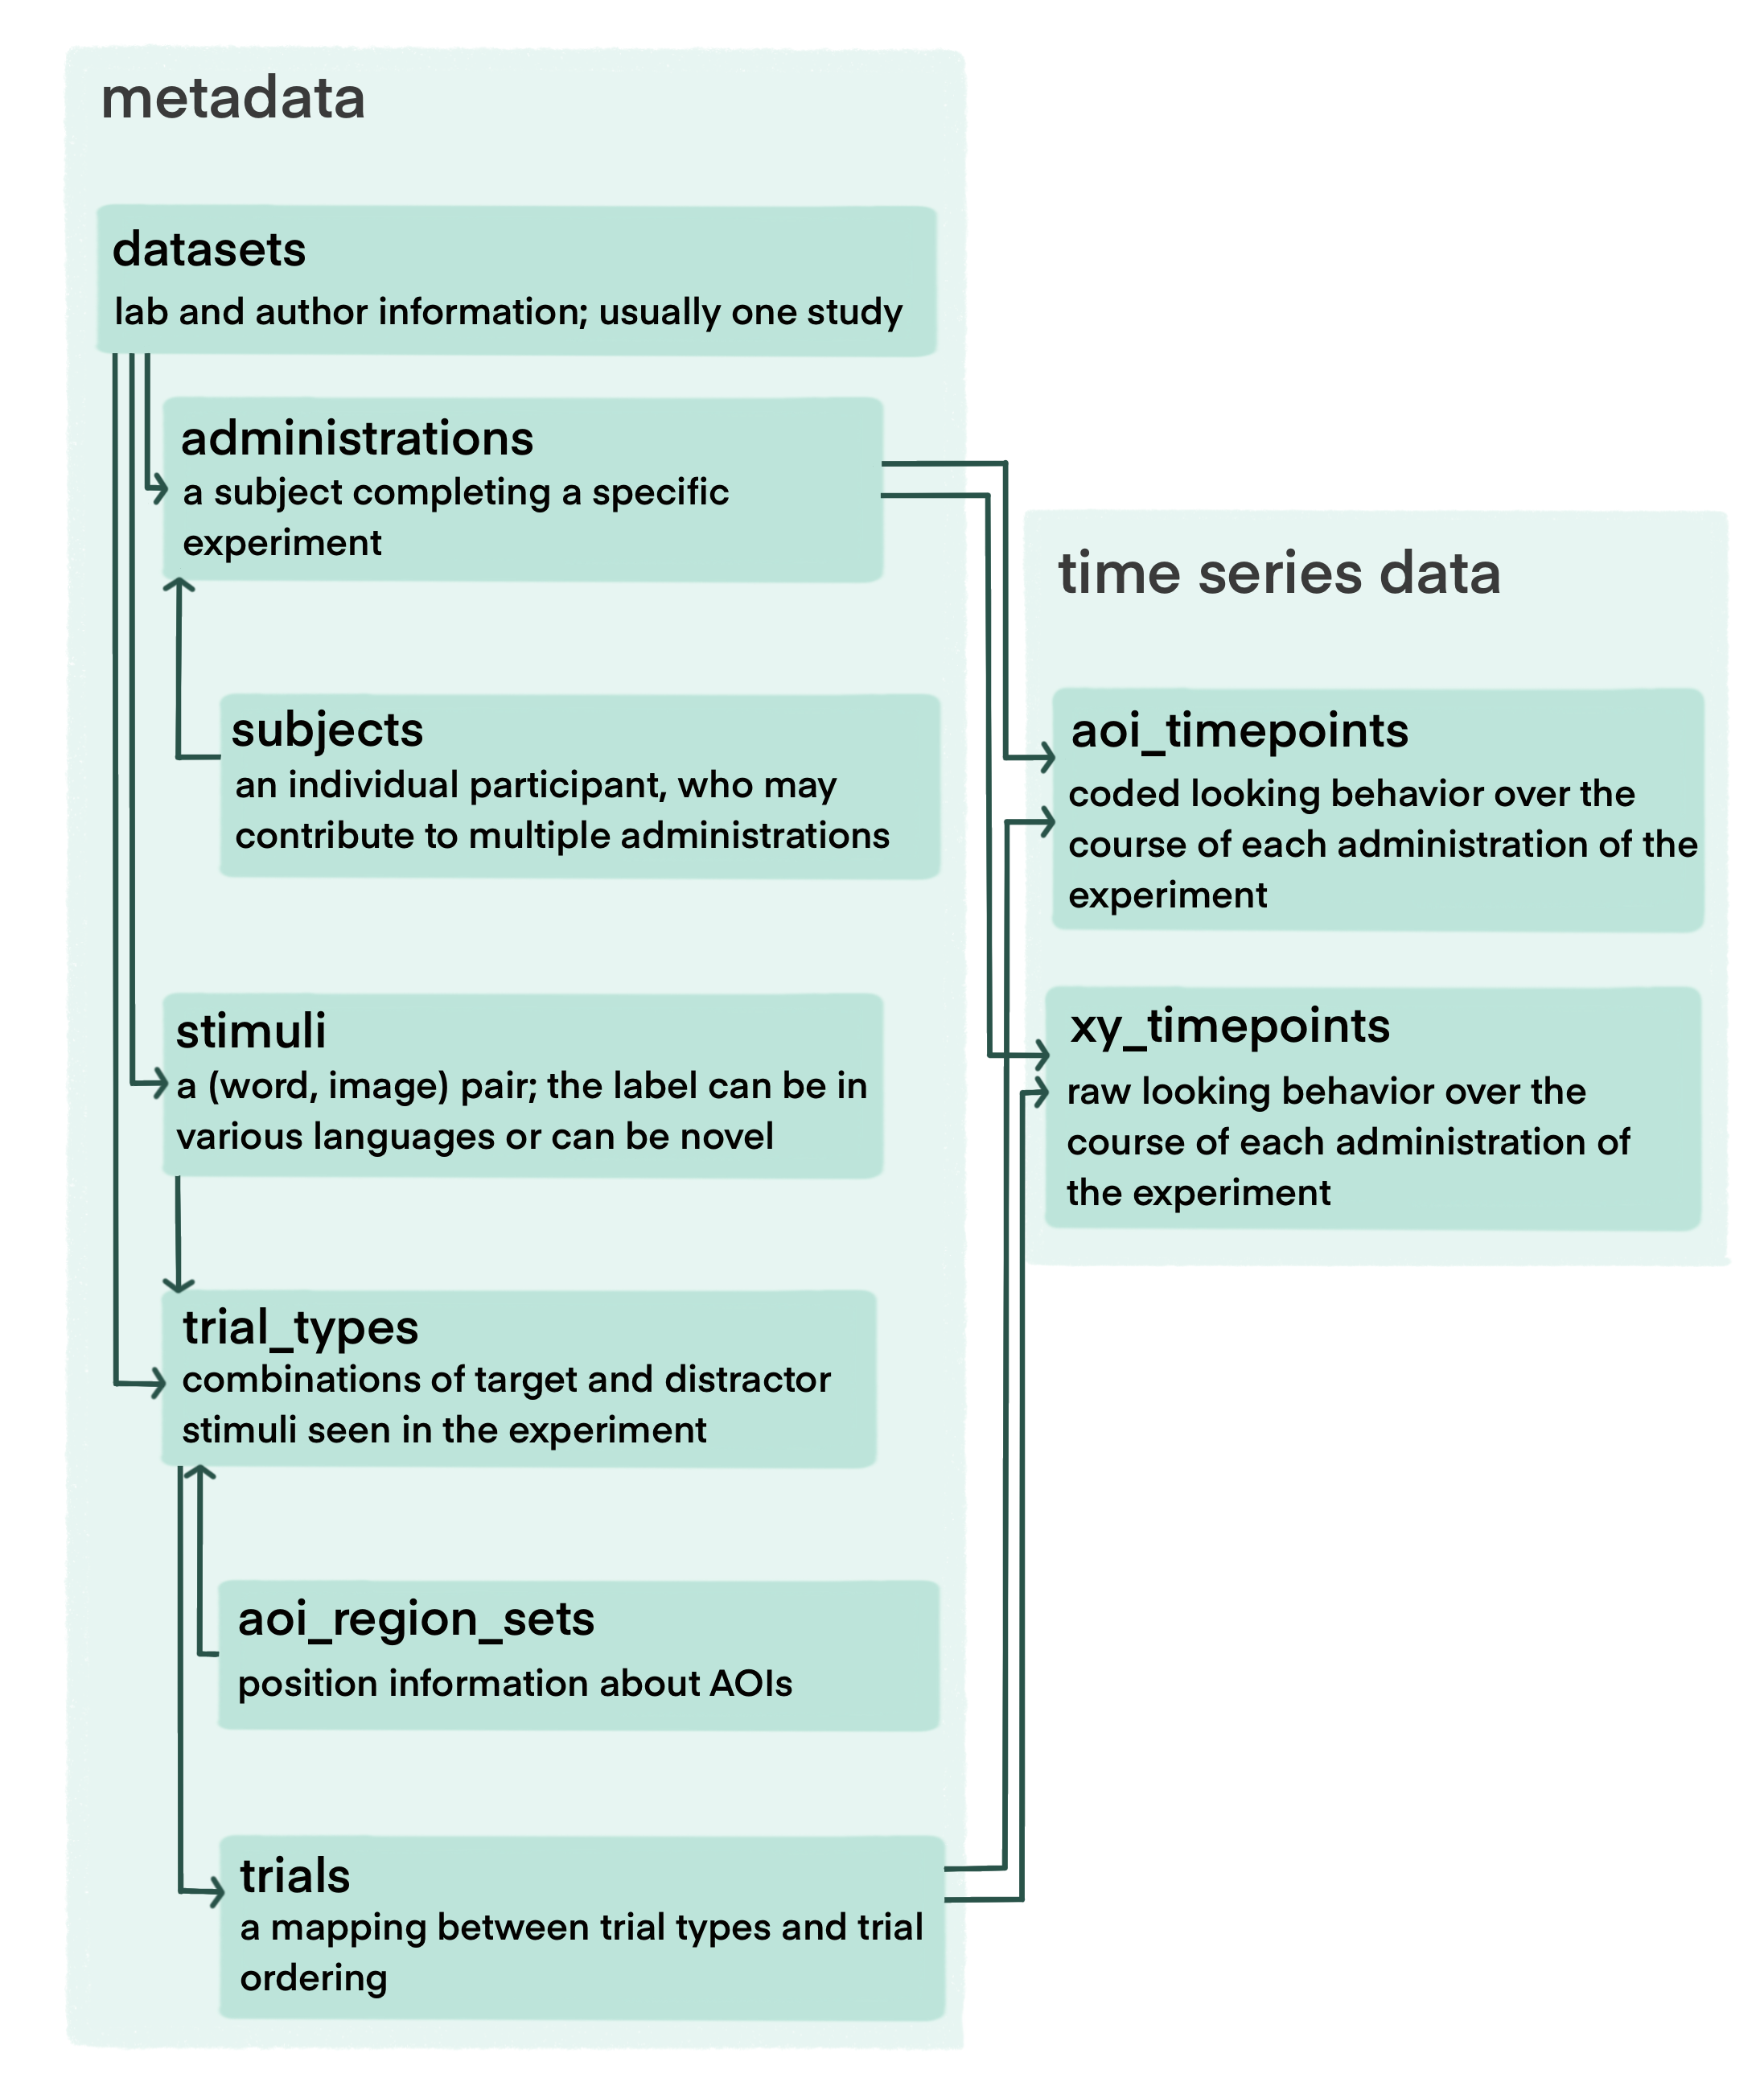
\includegraphics[width=7.31in,height=4.5in]{/Users/mikabr/Dropbox/projects/peekbank/peekbank-paper/brm/figures/schema_3} 

}

\caption{The Peekbank schema. Each square represents a table in the relational database.}\label{fig:fig-schema}
\end{figure}

\hypertarget{current-data-sources}{%
\subsection{Current Data Sources}\label{current-data-sources}}

\begin{table}[ht]
\centering
\begingroup\fontsize{9pt}{10pt}\selectfont
\scalebox{0.85}{
\begin{tabular}{lrrrrrr}
  \hline
Dataset Name & Citation & N & Mean Age (mos.) & Age Range (mos.) & Method & Language \\ 
  \hline
attword & (Yurovsky \& Frank, 2017) & 288 & 25.5 & 13 - 59 & eye-tracking & English \\ 
  canine & unpublished & 36 & 23.8 & 21 - 27 & manual coding & English \\ 
  coartic & (Mahr et al., 2015) & 29 & 20.8 & 18 - 24 & eye-tracking & English \\ 
  cowpig & (Perry et al., 2017) & 45 & 20.5 & 19 - 22 & manual coding & English \\ 
  ft\_pt & (Adams et al., 2018) & 69 & 17.1 & 13 - 20 & manual coding & English \\ 
  mispron & (Swingley \& Aslin, 2002) & 50 & 15.1 & 14 - 16 & manual coding & English \\ 
  mix & (Byers-Heinlein et al., 2017) & 48 & 20.1 & 19 - 21 & eye-tracking & English, French \\ 
  reflook\_socword & (Yurovsky et al., 2013) & 435 & 33.6 & 12 - 70 & eye-tracking & English \\ 
  reflook\_v4 & unpublished & 45 & 34.2 & 11 - 60 & eye-tracking & English \\ 
  remix & (Potter et al., 2019) & 44 & 22.6 & 18 - 29 & manual coding & Spanish, English \\ 
  salientme & (Pomper \& Saffran, 2019) & 44 & 40.1 & 38 - 43 & manual coding & English \\ 
  switchingCues & (Pomper \& Saffran, 2016) & 60 & 44.3 & 41 - 47 & manual coding & English \\ 
  tablet & (Frank et al., 2016) & 69 & 35.5 & 12 - 60 & eye-tracking & English \\ 
  tseltal & (Casillas et al., 2017) & 23 & 31.3 & 9 - 48 & manual coding & Tseltal \\ 
  yoursmy & (Garrison et al., 2020) & 35 & 14.5 & 12 - 18 & eye-tracking & English \\ 
   \hline
\end{tabular}
}
\endgroup
\caption{Overview over the datasets in the current database.} 
\end{table}

The database currently includes 11 looking-while-listening datasets comprising \emph{N}=1320 total participants (Table XX).
Most datasets (10 out of 11 total) consist of data from monolingual native English speakers.
They span a wide age spectrum with participants ranging from 8 to 84 months of age, and are balanced in terms of gender (48\% female).
The datasets vary across a number of dimensions related to design and methodology, and include studies using manually coded video recordings and automated eye-tracking methods (e.g., Tobii, EyeLink) to measure gaze behavior.
Most studies focused on testing familiar items, but the database also includes studies with novel pseudowords.
All data (and accompanying references) are openly available on the Open Science Framework (\url{https://osf.io/pr6wu/?view_only=07a3887eb7a24643bdc1b2612f2729de}).

How selected?
Language coverage?
More details about lab and design variation?

\hypertarget{versioning-expanding-the-database}{%
\subsection{Versioning + Expanding the database}\label{versioning-expanding-the-database}}

Information about versioning approach/ regularity of updates Steps for extending the database?

\hypertarget{interfacing-with-peekbank}{%
\section{Interfacing with peekbank}\label{interfacing-with-peekbank}}

\hypertarget{shiny-app}{%
\subsection{Shiny App}\label{shiny-app}}

One goal of the Peekbank project is to allow a wide range of users to easily explore and learn from the database.
We therefore have created an interactive web application -- \texttt{peekbank-shiny} -- that allows users to quickly and easily create informative visualizations of individual datasets and aggregated data.
\texttt{peekbank-shiny} is built using Shiny, a software package for creating web apps using R.
The Shiny app allows users to create commonly used visualizations of looking-while-listening data, based on data from the Peekbank database.
Specifically, users can visualize

\begin{enumerate}
\def\labelenumi{\arabic{enumi}.}
\tightlist
\item
  the time course of looking data in a profile plot depicting infant target looking across trial time
\item
  overall accuracy (proportion target looking) within a specified analysis window
\item
  reaction times (speed of fixating the target image) in response to a target label
\item
  an onset-contingent plot, which shows the time course of participant looking as a function of their look location at the onset of the target label
\end{enumerate}

Users are given various customization options for each of these visualizations, e.g., choosing which datasets to include in the plots, controlling the age range of participants, splitting the visualizations by age bins, and controlling the analysis window for time course analyses.
Plots are then updated in real time to reflect users' customization choices, and users are given options to share the visualizations they created.
The Shiny app thus allows users to quickly inspect basic properties of Peekbanks datasets and create reproducible visualizations without incurring any of the technical overhead required to access the database through R.

\hypertarget{peekbankr}{%
\subsection{Peekbankr}\label{peekbankr}}

Functions: connect\_to\_peekbank(): get\_datasets() get\_subjects() get\_administrations() get\_stimuli() get\_aoi\_timepoints() get\_trials() get\_trial\_types() get\_xy\_timepoints() get\_aoi\_region\_sets()

\hypertarget{osf-site}{%
\subsection{OSF site}\label{osf-site}}

Stimuli Data in raw format (if some additional datum needed, e.g.~pupil size?)

\hypertarget{peekbank-in-action}{%
\section{Peekbank in Action}\label{peekbank-in-action}}

We provide two potential use-cases for Peekbank data. In each case, we provide sample code so as to model how easy it is to do simple analyses using data from the database. Our first example shows how we can replicate the analysis for a classic study. This type of computational reproducibility can be a very useful exercise for teaching students about best practices for data analysis (e.g., Hardwicke et al., 2018) and also provides an easy way to explore looking-while-listening timecourse data in a standardized format. Our second example shows an in-depth exploration of developmental changes in the recognition of particular words. Besides its theoretical interest (which we will explore more fully in subsequent work), this type of analysis can be used for optimizing the stimuli for new experiments.

\hypertarget{computational-reproducibility-example-swingley2000}{%
\subsection{Computational reproducibility example: Swingley and Aslin (2000)}\label{computational-reproducibility-example-swingley2000}}

Swingley and Aslin (2000) investigated the specificity of 14-16 month-olds' word representations using the looking-while-listening paradigm, asking whether recognition would be slower and less accurate for mispronunciations, e.g.~``oppel'' (close mispronunciation) or ``opel'' (distant mispronunciation) instead of ``apple'' (correct condition). In this short vignette, we show how easily the data in Peekbank can be used to visualize this result.

\begin{Shaded}
\begin{Highlighting}[]
\NormalTok{aoi\_timepoints }\OtherTok{\textless{}{-}}\NormalTok{ peekbankr}\SpecialCharTok{::}\FunctionTok{get\_aoi\_timepoints}\NormalTok{(}\AttributeTok{dataset\_name =} \StringTok{"swingley\_aslin\_2002"}\NormalTok{)}
\NormalTok{administrations }\OtherTok{\textless{}{-}}\NormalTok{ peekbankr}\SpecialCharTok{::}\FunctionTok{get\_administrations}\NormalTok{(}\AttributeTok{dataset\_name =} \StringTok{"swingley\_aslin\_2002"}\NormalTok{)}
\NormalTok{trial\_types }\OtherTok{\textless{}{-}}\NormalTok{ peekbankr}\SpecialCharTok{::}\FunctionTok{get\_trial\_types}\NormalTok{(}\AttributeTok{dataset\_name =} \StringTok{"swingley\_aslin\_2002"}\NormalTok{)}
\NormalTok{trials }\OtherTok{\textless{}{-}}\NormalTok{ peekbankr}\SpecialCharTok{::}\FunctionTok{get\_trials}\NormalTok{(}\AttributeTok{dataset\_name =} \StringTok{"swingley\_aslin\_2002"}\NormalTok{)}
\end{Highlighting}
\end{Shaded}

We begin by retrieving the relevant tables from the database, \texttt{aoi\_timepoints}, \texttt{administrations}, \texttt{trial\_types}, and \texttt{trials}. As discussed above, each of these can be downloaded using a simple API call through \texttt{peekbankr}, which returns dataframes that include ID fields. These ID fields allow for easy joining of the data into a single dataframe containing all the information necessary for the analysis.

\begin{Shaded}
\begin{Highlighting}[]
\NormalTok{swingley\_data }\OtherTok{\textless{}{-}}\NormalTok{ aoi\_timepoints }\SpecialCharTok{\%\textgreater{}\%}
  \FunctionTok{left\_join}\NormalTok{(administrations) }\SpecialCharTok{\%\textgreater{}\%}
  \FunctionTok{left\_join}\NormalTok{(trials) }\SpecialCharTok{\%\textgreater{}\%}
  \FunctionTok{left\_join}\NormalTok{(trial\_types) }\SpecialCharTok{\%\textgreater{}\%}
  \FunctionTok{filter}\NormalTok{(condition }\SpecialCharTok{!=} \StringTok{"filler"}\NormalTok{) }\SpecialCharTok{\%\textgreater{}\%}
  \FunctionTok{mutate}\NormalTok{(}\AttributeTok{condition =} \FunctionTok{ifelse}\NormalTok{(condition }\SpecialCharTok{==} \StringTok{"cp"}\NormalTok{, }\StringTok{"Correct"}\NormalTok{,}\StringTok{"Mispronunciation"}\NormalTok{))}
\end{Highlighting}
\end{Shaded}

As the code above shows, once the data are joined, condition information for each timepoint is present and so we can easily filter out filler trials and set up the conditions for further analysis. For simplicity, here we combine both mispronunciation conditions since this manipulation showed no effect in the original paper.

\begin{Shaded}
\begin{Highlighting}[]
\NormalTok{accuracies }\OtherTok{\textless{}{-}}\NormalTok{ swingley\_data  }\SpecialCharTok{\%\textgreater{}\%}
  \FunctionTok{group\_by}\NormalTok{(t\_norm, administration\_id, condition) }\SpecialCharTok{\%\textgreater{}\%} 
  \FunctionTok{summarize}\NormalTok{(}\AttributeTok{correct =} \FunctionTok{mean}\NormalTok{(aoi }\SpecialCharTok{==} \StringTok{"target"}\NormalTok{) }\SpecialCharTok{/} 
              \FunctionTok{mean}\NormalTok{(aoi }\SpecialCharTok{\%in\%} \FunctionTok{c}\NormalTok{(}\StringTok{"target"}\NormalTok{,}\StringTok{"distractor"}\NormalTok{))) }\SpecialCharTok{\%\textgreater{}\%}
  \FunctionTok{group\_by}\NormalTok{(t\_norm, condition) }\SpecialCharTok{\%\textgreater{}\%} 
  \FunctionTok{summarize}\NormalTok{(}\AttributeTok{ci =} \FloatTok{1.96} \SpecialCharTok{*} \FunctionTok{sd}\NormalTok{(correct) }\SpecialCharTok{/} \FunctionTok{sqrt}\NormalTok{(}\FunctionTok{length}\NormalTok{(correct)), }
            \AttributeTok{mean\_correct =} \FunctionTok{mean}\NormalTok{(correct))}
\end{Highlighting}
\end{Shaded}

\begin{figure}
\centering
\includegraphics{peekbank-brm_files/figure-latex/swingley_fig-1.pdf}
\caption{(\#fig:swingley\_fig)Proportion looking at the correct referent by time from the point of disambiguation (the onset of the target noun). Colors show the two pronunciation conditions; points give means and ranges show 95\% confidence intervals. The dotted line shows the point of disambiguation and the dashed line shows chance performance.}
\end{figure}

The final step in our analysis is to create a summary dataframe using \texttt{dplyr} commands. We first group the data by timestep, participant, and condition and compute the proportion looking at the correct image. We then summarize again, averaging across participants, computing both means and 95\% confidence intervals (via the approximation of 1.96 times the standard error of the mean). The resulting dataframe can be used for visualization of the time-course of looking.

\begin{Shaded}
\begin{Highlighting}[]
\FunctionTok{ggplot}\NormalTok{(accuracies, }\FunctionTok{aes}\NormalTok{(}\AttributeTok{x =}\NormalTok{ t\_norm, }\AttributeTok{y =}\NormalTok{ mean\_correct, }\AttributeTok{col =}\NormalTok{ condition))}\SpecialCharTok{+}
  \FunctionTok{geom\_pointrange}\NormalTok{(}\FunctionTok{aes}\NormalTok{(}\AttributeTok{ymin =}\NormalTok{ mean\_correct }\SpecialCharTok{{-}}\NormalTok{ ci, }
                      \AttributeTok{ymax =}\NormalTok{ mean\_correct }\SpecialCharTok{+}\NormalTok{ ci))}
\end{Highlighting}
\end{Shaded}

Figure \ref{fig:swingley_fig} shows the average time course of looking for the two conditions, as produced by the code above (styling commands are removed for clarity of presentation, but are available in the Markdwon). Looks after the correctly pronounced noun appeared both faster (deviating from chance earlier) and more accurate (showing a higher asymptote). Overall, this example demonstrates the ability to produce this visualization in just a few lines of code.

\hypertarget{item-analyses}{%
\subsection{Item analyses}\label{item-analyses}}

To illustrate the power of aggregating data across multiple datasets, we,

aspirational goal -

ALso, item selection but maybe not yet?

\hypertarget{links-to-parent-report-vocabulary-data}{%
\subsection{Links to parent report vocabulary data}\label{links-to-parent-report-vocabulary-data}}

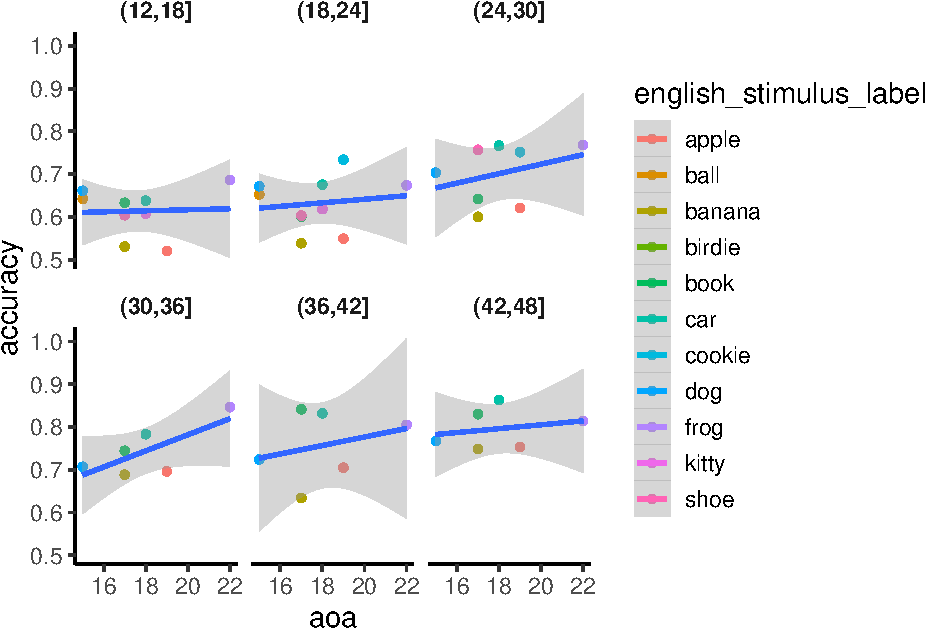
\includegraphics{peekbank-brm_files/figure-latex/aoas-1.pdf}

\hypertarget{discussion-conclusion}{%
\section{Discussion/ Conclusion}\label{discussion-conclusion}}

Theoretical progress in understanding child development requires rich datasets, but collecting child data is expensive, difficult, and time-intensive.
Recent years have seen a growing effort to build open source tools and pool research efforts to meet the challenge of building a cumulative developmental science (Bergmann et al. (2018); Frank, Braginsky, Yurovsky, and Marchman (2017); The ManyBabies Consortium (2020){]}.
The Peekbank project expands on these efforts by building an infrastructure for aggregating eye-tracking data across studies, with a specific focus on the looking-while-listening paradigm.
This paper presents an illustration of some of the key theoretical and methodological questions that can be addressed using Peekbank: generalizing across item-level variability in children's word recognition and providing data-driven guidance on methodological choices.

There are a number of limitations surrounding the current scope of the database.
A priority in future work will be to expand the size of the database.
With 11 datasets currently available in the database, idiosyncrasies of particular designs and condition manipulations still have substantial influence on modeling results.
Expanding the set of distinct datasets will allow us to increase the number of observations per item across datasets, leading to more robust generalizations across item-level variability.
The current database is also limited by the relatively homogeneous background of its participants, both with respect to language (almost entirely monolingual native English speakers) and cultural background (all but one dataset comes from WEIRD populations; (Muthukrishna et al., 2020).
Increasing the diversity of participant backgrounds and languages will expand the scope of the generalizations we can form about child word recognition.

Finally, while the current database is focused on studies of word recognition, the tools and infrastructure developed in the project can in principle be used to accommodate any eye-tracking paradigm, opening up new avenues for insights into cognitive development.
Gaze behavior has been at the core of many of the key advances in our understanding of infant cognition.
Aggregating large datasets of infant looking behavior in a single, openly-accessible format promises to bring a fuller picture of infant cognitive development into view.

\hypertarget{acknowledgements}{%
\section{Acknowledgements}\label{acknowledgements}}

We would like to thank the labs and researchers that have made their data publicly available in the database.

We used R {[}Version 4.1.0; R Core Team (2020){]} for all our analyses.

\newpage

\hypertarget{references}{%
\section{References}\label{references}}

\begingroup
\setlength{\parindent}{-0.5in}
\setlength{\leftskip}{0.5in}

\hypertarget{refs}{}
\begin{CSLReferences}{1}{0}
\leavevmode\hypertarget{ref-bergelson2020}{}%
Bergelson, E. (2020). The comprehension boost in early word learning: Older infants are better learners. \emph{Child Development Perspectives}, \emph{14}(3), 142--149.

\leavevmode\hypertarget{ref-bergelson2012}{}%
Bergelson, E., \& Swingley, D. (2012). {At 6-9 months, human infants know the meanings of many common nouns.} \emph{PNAS}, \emph{109}(9), 3253--3258.

\leavevmode\hypertarget{ref-bergmann2018}{}%
Bergmann, C., Tsuji, S., Piccinini, P. E., Lewis, M. L., Braginsky, M., Frank, M. C., \& Cristia, A. (2018). {Promoting replicability in developmental research through meta-analyses: Insights from language acquisition research}. \emph{Child Development}, \emph{89}(6), 1996--2009.

\leavevmode\hypertarget{ref-bleses2016}{}%
Bleses, D., Makransky, G., Dale, P. S., Højen, A., \& Ari, B. A. (2016). {Early productive vocabulary predicts academic achievement 10 years later}. \emph{Applied Psycholinguistics}, \emph{37}(6), 1461--1476.

\leavevmode\hypertarget{ref-csibra2016}{}%
Csibra, G., Hernik, M., Mascaro, O., Tatone, D., \& Lengyel, M. (2016). {Statistical treatment of looking-time data}. \emph{Developmental Psychology}, \emph{52}(4), 521--536.

\leavevmode\hypertarget{ref-fernald2012}{}%
Fernald, A., \& Marchman, V. A. (2012). {Individual differences in lexical processing at 18 months predict vocabulary growth in typically developing and late-talking toddlers.} \emph{Child Development}, \emph{83}(1), 203--222.

\leavevmode\hypertarget{ref-fernald1998}{}%
Fernald, A., Pinto, J. P., Swingley, D., Weinberg, A., \& McRoberts, G. W. (1998). Rapid gains in speed of verbal processing by infants in the 2nd year. \emph{Psychological Science}, \emph{9}(3), 228--231.

\leavevmode\hypertarget{ref-fernald2008}{}%
Fernald, A., Zangl, R., Portillo, A. L., \& Marchman, V. A. (2008). {Looking while listening: Using eye movements to monitor spoken language comprehension by infants and young children}. In I. A. Sekerina, E. M. Fernandez, \& H. Clahsen (Eds.), \emph{Developmental psycholinguistics: On-line methods in children's language processing} (pp. 97--135). Amsterdam: John Benjamins.

\leavevmode\hypertarget{ref-frank2017}{}%
Frank, M. C., Braginsky, M., Yurovsky, D., \& Marchman, V. A. (2017). {Wordbank: An open repository for developmental vocabulary data}. \emph{Journal of Child Language}, \emph{44}(3), 677--694.

\leavevmode\hypertarget{ref-frank2021}{}%
Frank, M. C., Braginsky, M., Yurovsky, D., \& Marchman, V. A. (2021). \emph{{Variability and Consistency in Early Language Learning: The Wordbank Project}}. Cambridge, MA: MIT Press.

\leavevmode\hypertarget{ref-golinkoff2013}{}%
Golinkoff, R. M., Ma, W., Song, L., \& Hirsh-Pasek, K. (2013). {Twenty-five years using the intermodal preferential looking paradigm to study language acquisition: What have we learned?} \emph{Perspectives on Psychol. Science}, \emph{8}(3), 316--339.

\leavevmode\hypertarget{ref-hardwicke2018}{}%
Hardwicke, T. E., Mathur, M. B., MacDonald, K., Nilsonne, G., Banks, G. C., Kidwell, M. C., \ldots{} Frank, M. C. (2018). {Data availability, reusability, and analytic reproducibility: Evaluating the impact of a mandatory open data policy at the journal Cognition}. \emph{Royal Society Open Science}, \emph{5}(8). \url{https://doi.org/10.1098/rsos.180448}

\leavevmode\hypertarget{ref-hirshpasek1987}{}%
Hirsh-Pasek, K., Cauley, K. M., Golinkoff, R. M., \& Gordon, L. (1987). {The eyes have it: Lexical and syntactic comprehension in a new paradigm}. \emph{Journal of Child Language}, \emph{14}(1), 23--45.

\leavevmode\hypertarget{ref-huang2020}{}%
Huang, Y., \& Snedeker, J. (2020). {Evidence from the visual world paradigm raises questions about unaccusativity and growth curve analyses}. \emph{Cognition}, \emph{200}, 104251.

\leavevmode\hypertarget{ref-lewwilliams2007}{}%
Lew-Williams, C., \& Fernald, A. (2007). {Young children learning Spanish make rapid use of grammatical gender in spoken word recognition}. \emph{Psychological Science}, \emph{18}(3), 193--198.

\leavevmode\hypertarget{ref-marchman2008}{}%
Marchman, V. A., \& Fernald, A. (2008). {Speed of word recognition and vocabulary knowledge in infancy predict cognitive and language outcomes in later childhood.} \emph{Developmental Science}, \emph{11}(3), F9--16.

\leavevmode\hypertarget{ref-marchman2018}{}%
Marchman, V. A., Loi, E. C., Adams, K. A., Ashland, M., Fernald, A., \& Feldman, H. M. (2018). {Speed of language comprehension at 18 months old predicts school-relevant outcomes at 54 months old in children born preterm}. \emph{Journal of Dev. {\&} Behav. Pediatrics}, \emph{39}(3), 246--253.

\leavevmode\hypertarget{ref-muthukrishna2020}{}%
Muthukrishna, M., Bell, A. V., Henrich, J., Curtin, C. M., Gedranovich, A., McInerney, J., \& Thue, B. (2020). {Beyond Western, Educated, Industrial, Rich, and Democratic (WEIRD) Psychology: Measuring and Mapping Scales of Cultural and Psychological Distance}. \emph{Psychological Science}, \emph{31}(6), 678--701.

\leavevmode\hypertarget{ref-peter2019}{}%
Peter, M. S., Durrant, S., Jessop, A., Bidgood, A., Pine, J. M., \& Rowland, C. F. (2019). Does speed of processing or vocabulary size predict later language growth in toddlers? \emph{Cognitive Psychology}, \emph{115}, 101238.

\leavevmode\hypertarget{ref-R-base}{}%
R Core Team. (2020). \emph{R: A language and environment for statistical computing}. Vienna, Austria: R Foundation for Statistical Computing. Retrieved from \url{https://www.R-project.org/}

\leavevmode\hypertarget{ref-swingley2000}{}%
Swingley, D., \& Aslin, R. N. (2000). {Spoken word recognition and lexical representation in very young children.} \emph{Cognition}, \emph{76}(2), 147--166.

\leavevmode\hypertarget{ref-manybabies2020}{}%
The ManyBabies Consortium. (2020). {Quantifying sources of variability in infancy research using the infant-directed speech preference}. \emph{Advances in Methods and Practices in Psychological Science}, \emph{3}(1), 24--52.

\end{CSLReferences}

\endgroup


\end{document}
